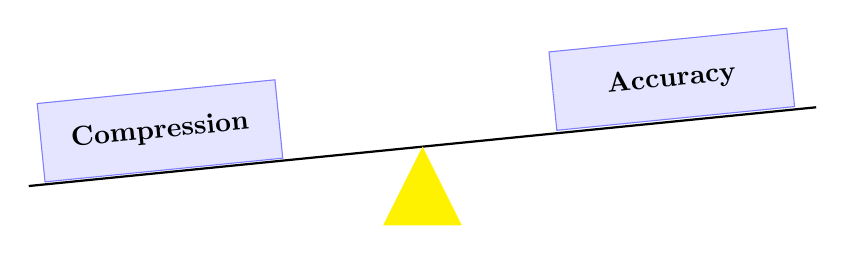
\begin{tikzpicture}

    % Seesaw beam (tilted from -5 to 5)
    \draw[thick] (-5,-0.5) -- (5,0.5);
    
    % Fulcrum (yellow triangle)
    \fill[yellow] (0,0) -- (-0.5,-1) -- (0.5,-1) -- cycle;

    % Rotation angle to match the beam tilt
    \def\tiltangle{5.7} % positive to match the upward slope from left to right

    % Left box - Compression (rotated to match beam angle)
    \node[draw=blue!50, fill=blue!10, text width=2.8cm, minimum height=1cm,
          align=center, anchor=south west, rotate=\tiltangle] at (-4.8,-0.455) {\textbf{Compression}};
    
    % Right box - Accuracy (rotated to match beam angle)
    \node[draw=blue!50, fill=blue!10, text width=2.8cm, minimum height=1cm,
          align=center, anchor=south west, rotate=\tiltangle] at (1.7,0.2) {\textbf{Accuracy}};
    
    
\end{tikzpicture}